\section{面向对象设计}
\label{sec:oodesign}

\begin{frame}
  \begin{center}
    \Huge{\textcolor{red}{面向对象设计}}
  \end{center}
\end{frame}

\subsection{迭代1}

\begin{frame}{需求}
  \begin{block}{}
    \begin{enumerate}
      \item<alert@1-> 需求1:判断某个单词是否包含数字
    \end{enumerate}
  \end{block}
\end{frame}

\begin{frame}[fragile]{快速实现:坏味道}
  \begin{c++}
  bool hasDigit(const string& word) {
    string::const_iterator i = word.begin();
    for (; i != word.end(); ++i)
      if (isdigit(*i))
        return true;
    return false;
  }
  \end{c++}

  \begin{itemize}
    \item \alert{坏味道}
  \end{itemize} 
\end{frame}

\begin{frame}[fragile]{类型推演}
  \begin{c++}
  bool hasDigit(const string& word) {
    for (auto c : word)
      if (isdigit(c))
        return true;
    return false;
  }
  \end{c++}

  \begin{itemize}
    \item \alert{意图明确}
    \item \alert{关注性能}
    \item \alert{消除冗余噪声}
    \item \alert{增强编译时安全}
  \end{itemize}
\end{frame}

\subsection{迭代2}

\begin{frame}{需求}
  \begin{block}{}
    \begin{enumerate}
    \item \alert{需求1}:判断某个单词是否包含数字
    \item<alert@1-> 需求2:判断某个单词是否包含大写字母
    \end{enumerate}
  \end{block}
\end{frame}

\begin{frame}[fragile]{重复设计:复制 \& 粘贴}
  \begin{c++}
  bool hasUpper(const string& word) {
    for (auto c : word)
      if (isupper(c))
        return true;
    return false;
  }
  \end{c++}

  \begin{itemize}
    \item \alert{消除重复}
    \item \alert{分离变化}
  \end{itemize}    
\end{frame}

\begin{frame}[fragile]{DRY}
  \begin{figure}
    \centering
    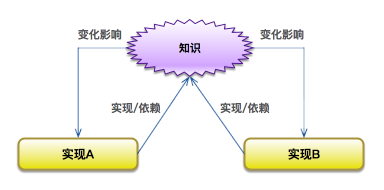
\includegraphics[width=0.7\textwidth]{dry.png}
  \end{figure}
\end{frame}

\begin{frame}[fragile]{抽象}
  \begin{c++}
  template <typename Matcher>
  bool exists(const string& word, Matcher matcher) {
    for (auto c : word)
      if (matcher(c))
        return true;
    return false;
  }  
  \end{c++}

  \begin{itemize}
    \item \alert{愿意被第一颗子弹击中,但拒绝同一方向的子弹再次被击中}
    \item \alert{愚弄我一次,应感羞愧的是你;再次愚弄我,应感羞愧的是我}
    \item \alert{没有一种设计是永远\ascii{OCP},只存在对当前变化保持\ascii{OCP}}
  \end{itemize}
\end{frame}

\begin{frame}[fragile]{泛化}
  \begin{c++}
  template <typename Iterator, typename Matcher>
  bool exists(Iterator first, Iterator last, Matcher matcher) {
    for (; first != last; ++first)
      if (matcher(*first))
        return true;
    return false;
  }
  \end{c++}

  \begin{itemize}
    \item \alert{容器类型}
    \item \alert{迭代算法}
    \item \alert{匹配准则}    
  \end{itemize}
\end{frame}

\begin{frame}[fragile]{无参函数对象}
\begin{columns} 
  \begin{column}{0.7\textwidth}
  \begin{c++}
  struct {
    bool operator()(char c) const {
      return std::isdigit(c); 
    }
  } is_digit;

  struct {
    bool operator()(char c) const {
      return std::isupper(c); 
    }
  } is_upper;

  exists(word.begin(), word.end(), is_digit);
  exists(word.begin(), word.end(), is_upper);
  \end{c++}
  \end{column} 

  \begin{column}{0.3\textwidth}
  \begin{itemize}
    \item \alert{组合小类}
    \item \alert{复用对象}
  \end{itemize}  
  \end{column}
  \end{columns} 
\end{frame}

\subsection{迭代3}

\begin{frame}{需求}
  \begin{block}{}
    \begin{enumerate}
    \item \alert{需求1}:判断某个单词是否包含数字
    \item \alert{需求2}:判断某个单词是否包含大写字母
    \item<alert@1-> 需求3:判断某个单词是否包含下划线 
    \end{enumerate}
  \end{block}
\end{frame}

\begin{frame}[fragile]{有参函数对象}
  \begin{c++}
  template <typename T>
  struct Equals {
    explicit Equals(const T& t) : t(t)
    {}

    bool operator()(const T& t) const {
      return this->t == t;
    }

  private:
    T t;
  };

  exists(word.begin(), word.end(), Equals<char>('_'));
  \end{c++}

  \begin{itemize}
    \item \alert{心智包袱}
  \end{itemize}
\end{frame}

\begin{frame}[fragile]{工厂方法:equals\_to}
  \begin{c++}
  template <typename T>
  auto equals_to(const T& t) {
    return Equals<T>(t);
  }

  exists(word.begin(), word.end(), equals_to('_'));
  \end{c++}

  \begin{itemize}
    \item \alert{类型推演}    
    \item \alert{零负担}
  \end{itemize}  
\end{frame}

\begin{frame}[fragile]{实用对象}
  \begin{c++}
  const Equals<std::string> is_empty("");
  const Equals<const void*> is_nil(nullptr);
  \end{c++}

  \begin{itemize}
    \item \alert{语法糖}    
    \item \alert{复用对象}
  \end{itemize}  
\end{frame}

\subsection{迭代4}

\begin{frame}{需求}
  \begin{block}{}
    \begin{enumerate}
    \item \alert{需求1}:判断某个单词是否包含数字
    \item \alert{需求2}:判断某个单词是否包含大写字母
    \item \alert{需求3}:判断某个单词是否包含下划线 
    \item<alert@1-> 需求4:判断某个单词是否不包含下划线     
    \end{enumerate}
  \end{block}
\end{frame}

\begin{frame}[fragile]{修饰语义}
\begin{columns} 
  \begin{column}{0.8\textwidth}
  \begin{c++}
  template <typename Matcher>
  struct Not {
    Not(const Matcher& matcher)
      : matcher(matcher)
    {}

    template <typename T>
    bool operator()(const T& actual) const {
      return !matcher(actual);
    }

  private:
    Matcher matcher;
  };
  \end{c++}
  \end{column}

  \begin{column}{0.2\textwidth}
  \begin{itemize}
    \item \alert{修饰语义}
    \item \alert{增强功能}
  \end{itemize}      
  \end{column}
\end{columns}   
\end{frame}

\begin{frame}[fragile]{工厂方法: is\_not}
  \begin{c++}
  template <typename Matcher>
  auto is_not(const Matcher& matcher) {
    return Not<Matcher>(matcher);
  }  

  forall(word.begin(), word.end(), is_not(equals_to('_')));
  \end{c++}
\end{frame}

\begin{frame}[fragile]{重复再现}
  \begin{c++}
  template <typename Iterator, typename Matcher>
  bool exists(Iterator first, Iterator last, Matcher matcher) {
    for (; first != last; ++first)
      if (matcher(*first))
        return true;
    return false;
  }

  template <typename Iterator, typename Matcher>
  bool forall(Iterator first, Iterator last, Matcher matcher) {
    for (; first != last; ++first)
      if (!matcher(*first))
        return false;
    return true;
  }
  \end{c++}
\end{frame}

\begin{frame}[fragile]{提取函数}
  \begin{c++}
  template <bool shortcut, typename Iterator, typename Matcher>
  bool expect(Iterator first, Iterator last, Matcher matcher) {
    for (; first != last; ++first)
      if (matcher(*first) == shortcut)
        return shortcut;
    return !shortcut;
  }

  template <typename Iterator, typename Matcher>
  bool exists(Iterator first, Iterator last, Matcher matcher) {
    return expect<true>(first, last, matcher);
  }

  template <typename Iterator, typename Matcher>
  bool forall(Iterator first, Iterator last, Matcher matcher) {
    return expect<false>(first, last, matcher);
  }
  \end{c++}
\end{frame}

\subsection{迭代5}

\begin{frame}{需求}
  \begin{block}{}
    \begin{enumerate}
    \item \alert{需求1}:判断某个单词是否包含数字
    \item \alert{需求2}:判断某个单词是否包含大写字母
    \item \alert{需求3}:判断某个单词是否包含下划线 
    \item \alert{需求4}:判断某个单词是否不包含\_
    \item<alert@1-> 需求5:判断某个单词是否包含\_,或者*
    \end{enumerate}
  \end{block}
\end{frame}

\begin{frame}[fragile]{组合或}
  \begin{c++}
  template <typename LeftMatcher, typename RightMatcher>
  struct Or {
    Or(const LeftMatcher& left, const RightMatcher& right)
      : left(left), right(right) {
    }

    template <typename T>
    bool operator()(const T& actual) const {
      return left(actual) || right(actual);
    }

  private:
    LeftMatcher  left;
    RightMatcher right;
  };
  \end{c++}
\end{frame}

\begin{frame}[fragile]{组合或:工厂}
  \begin{c++}
  template <typename LeftMatcher, typename RightMatcher>
  auto is_or(const LeftMatcher& left, const RightMatcher& right) {
    return Or<LeftMatcher, RightMatcher>(left, right);
  }

  exists(word.begin(), word.end(), is_or(
    equals_to('_'), equals_to('*')
  )); 
  \end{c++}
\end{frame}

\subsection{迭代6}

\begin{frame}{需求}
  \begin{block}{}
    \begin{enumerate}
    \item \alert{需求1}:判断某个单词是否包含数字
    \item \alert{需求2}:判断某个单词是否包含大写字母
    \item \alert{需求3}:判断某个单词是否包含下划线 
    \item \alert{需求4}:判断某个单词是否不包含\_
    \item \alert{需求5}:判断某个单词是否包含\_,或者\*     
    \item<alert@1-> 需求6:判断某个单词是否包含空白符,但除去空格     
    \end{enumerate}
  \end{block}
\end{frame}

\begin{frame}[fragile]{组合与}
  \begin{c++}
  template <typename LeftMatcher, typename RightMatcher>
  struct And {
    And(const LeftMatcher& left, const RightMatcher& right)
      : left(left), right(right) {
    }

    template <typename T>
    bool operator()(const T& actual) const {
      return left(actual) && right(actual);
    }

  private:
    LeftMatcher  left;
    RightMatcher right;
  };
  \end{c++}
\end{frame}


\begin{frame}[fragile]{工厂:组合与}
  \begin{c++}
  template <typename LeftMatcher, typename RightMatcher>
  auto is_and(const LeftMatcher& left, const RightMatcher& right) {
    return And<LeftMatcher, RightMatcher>(left, right);
  }

  exists(word.begin(), word.end(), is_and( 
    is_space, is_not(equals_to(' ')) 
  ));
  \end{c++}
\end{frame}

\subsection{迭代7}

\begin{frame}{需求}
  \begin{block}{}
    \begin{enumerate}
    \item \alert{需求1}:判断某个单词是否包含数字
    \item \alert{需求2}:判断某个单词是否包含大写字母
    \item \alert{需求3}:判断某个单词是否包含下划线 
    \item \alert{需求4}:判断某个单词是否不包含\_
    \item \alert{需求5}:判断某个单词是否包含\_,或者\*     
    \item \alert{需求6}:判断某个单词是否包含空白符,但除去空格
    \item<alert@1-> 需求7:判断某个单词是否包含字母x,且不区分大小写
    \end{enumerate}
  \end{block}
\end{frame}

\begin{frame}[fragile]{修饰}
  \begin{c++}
  template <typename Matcher, typename T>
  struct IgnoringCase {
    explicit IgnoringCase(const T& expect)
      : matcher(toLower(expect))
    {}

    bool operator()(const T& actual) const {
      return matcher(toLower(actual));
    }

  private:
    Matcher matcher;
  };
  \end{c++}
\end{frame}

\begin{frame}[fragile]{引入工厂}
  \begin{c++}
  template <typename T>
  auto ignoring_case_equals(const T& expected) {
    return IgnoringCase<Equals<T>, T>(expected);
  }  

  exists(word.begin(), word.end(), ignoring_case_equals('x'));
  \end{c++}
\end{frame}

\subsection{迭代8}

\begin{frame}{需求}
  \begin{block}{}
    \begin{enumerate}
    \item \alert{需求1}:判断某个单词是否包含数字
    \item \alert{需求2}:判断某个单词是否包含大写字母
    \item \alert{需求3}:判断某个单词是否包含下划线 
    \item \alert{需求4}:判断某个单词是否不包含\_
    \item \alert{需求5}:判断某个单词是否包含\_,或者\*     
    \item \alert{需求6}:判断某个单词是否包含空白符,但除去空格
    \item \alert{需求7}:判断某个单词是否包含字母x,且不区分大小写
    \item<alert@1-> 需求8:判断某个单词序列以子串开头(或结尾),且不区分大小写    
    \end{enumerate}
  \end{block}
\end{frame}

\begin{frame}[fragile]{字符串:Starts}
  \begin{c++}
  struct Starts {
    explicit Starts(const std::string& prefix) : prefix(prefix)
    {}

    bool operator()(const std::string& str) const {
      return str.length() >= prefix.length() &&
        str.compare(0, prefix.length(), prefix) == 0;
    }

  private:
    std::string prefix;
  };
  \end{c++}
\end{frame}

\begin{frame}[fragile]{字符串:Ends}
  \begin{c++}
  struct Ends {
    explicit Ends(const std::string& postfix) : postfix(postfix)
    {}

    bool operator()(const std::string& str) const {
      return str.length() >= postfix.length() &&
        str.compare(str.length() - postfix.length(), 
          postfix.length(), postfix) == 0;
    }

  private:
    std::string postfix;
  };
  \end{c++}
\end{frame}

\begin{frame}[fragile]{复用}
  \begin{c++}
  template <typename T>
  auto ignoring_case_starts(const T& prefix) {
    return IgnoringCase<Starts, string>(prefix);
  }  

  template <typename T>
  auto ignoring_case_ends(const T& postfix) {
    return IgnoringCase<Ends, string>(postfix);
  }  

  exists(words.begin(), words.end(), ignoring_case_starts("abc"));
  exists(words.begin(), words.end(), ignoring_case_ends("xyz"));  
  \end{c++}
\end{frame}

\subsection{迭代9}

\begin{frame}{需求}
  \begin{block}{}
    \begin{enumerate}
    \item \alert{需求1}:判断某个单词是否包含数字
    \item \alert{需求2}:判断某个单词是否包含大写字母
    \item \alert{需求3}:判断某个单词是否包含下划线 
    \item \alert{需求4}:判断某个单词是否不包含\_
    \item \alert{需求5}:判断某个单词是否包含\_,或者\*     
    \item \alert{需求6}:判断某个单词是否包含空白符,但除去空格
    \item \alert{需求7}:判断某个单词是否包含字母x,且不区分大小写
    \item \alert{需求8}:判断某个单词序列以子串开头(或结尾),且不区分大小写        
    \item<alert@1-> 需求9:判断某个单词满足某种特征,总是成功或失败    
    \end{enumerate}
  \end{block}
\end{frame}

\begin{frame}[fragile]{占位符}
  \begin{c++}
  template <bool value, typename T>
  struct Placeholder {
    bool operator()(const T&) const {
      return value;
    }
  };

  template <typename T>
  auto always() {
    return Placeholder<true, T>();
  }

  template <typename T>
  auto never() {
    return Placeholder<false, T>();
  }

  forall(word.begin(), word.end(), always<char>());  
  \end{c++}
\end{frame}

\begin{frame}[fragile]{领域模型}
  \begin{figure}
    \centering
    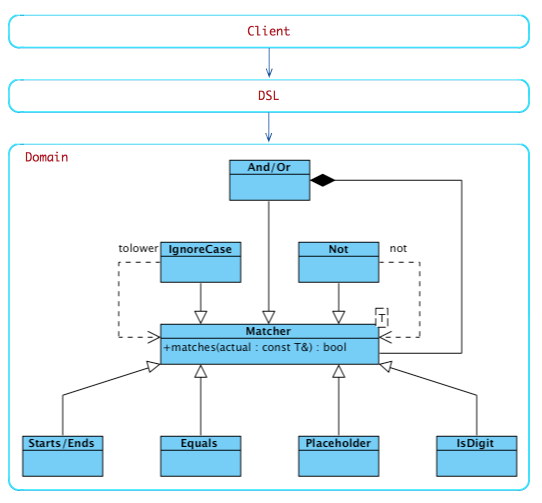
\includegraphics[width=0.6\textwidth]{matchers-model.png}
  \end{figure}
\end{frame}